\section{Results}

\subsection{Pointwise accuracy does not order long-time fidelity}

We first asked whether the conventional training objective---one-step displacement or velocity
error on held-out transitions---predicts the long-time behaviour of a force-free propagator. We
compared two models trained on the same SPC/Fw water data: our 250k relational propagator and the
published TrajCast water checkpoint. On 1,250 held-out transitions, the published checkpoint has a
mean absolute position error of \(4.75\times10^{-3}\) \AA{} and a velocity error of
\(1.63\times10^{-3}\) \AA{} fs\(^{-1}\). The 250k model is about fifteen times more accurate
pointwise (\(2.97\times10^{-4}\) \AA{} and \(1.09\times10^{-4}\) \AA{} fs\(^{-1}\)). If one-step
accuracy controlled long-time fidelity, the 250k model should be the better sampler.

It is not. Under the same 100 ps NVT protocol (300 K, CSVR, 5 fs), the published checkpoint
reproduces the canonical kinetic partition---translation \(2.505\) eV, rotation \(2.463\) eV,
internal \(2.444\) eV against the 2.5 ns reference means of \(2.459\), \(2.502\), and \(2.450\)
eV (the first 100 ps reference block is an outlier at \(2.373/2.430/2.609\) eV)---and gives
O--O, O--H, and H--H RDF RMSEs of 0.043, 0.118, and 0.096. The 250k model, despite its lower
one-step error, collapses the collective modes and overheats the internal mode: translation
\(0.538\) eV, rotation \(0.786\) eV, internal \(6.044\) eV. Its RDF RMSEs are 0.646, 1.312, and
0.249. The total kinetic energy is close to the target in both cases; the distribution across
modes is not. A pointwise-better model is a worse sampler, and the failure is invisible to the
training loss.

The inversion is not a peculiarity of one checkpoint. A 20k-step prefix of the same architecture
is even more pointwise accurate but becomes unstable in NVT after about 50 ps. A native TrajCast
architecture trained to only about 10\% of its schedule has a pointwise error three times smaller
than the 250k model and fails in the opposite direction---translation \(3.256\) eV, rotation
\(3.105\) eV, internal \(1.041\) eV. The sign of the mode bias is architecture- and
training-dependent, but its presence is not.

\subsection{NVE energy drift is a red herring}

A natural second hypothesis is that the failing models inject energy and heat, and that a better
energy integrator would fix the ensemble. We tested this directly with 25 ps NVE rollouts from the
same initial state. The published checkpoint heats from 302 K to 476 K; the 250k model cools from
302 K to 271 K; the NVT-pair fine-tuned M0 model heats to 387 K. The ordering by NVE drift is
essentially the reverse of the ordering by NVT fidelity: the model that heats the most passes the
NVT screen, and the most NVE-stable model fails it. Energy conservation and canonical sampling are
different properties of the composed map. A force-free propagator can be a poor energy integrator
and a good thermostat, or vice versa; NVE drift cannot be used as a surrogate for the stationary
measure.

\subsection{The failure is a mode-resolved partition bias}

The two diagnostics point to a common variable: the distribution of kinetic energy among molecular
modes. Figure~\ref{fig:diagnostic}c shows the mode kinetic energy relative to the reference for all
models. The failing models are not simply hot or cold. They are partitioned: the 250k family is
collectively cold and internally hot (translation 0.23, rotation 0.32, internal 2.32 of the
reference), the native/M0 family is collectively hot and internally cold (1.37, 1.28, 0.40), and
the published checkpoint is close to the reference on all three (1.06, 1.01, 0.94). The total
temperature is approximately 300 K in every case. A global thermostat holds the scalar temperature
while leaving the vector of mode temperatures biased.

This resolves the apparent paradox. The one-step loss is dominated by the conditional mean of the
displacement, which is insensitive to a slow redistribution of kinetic energy across modes. The
NVE trajectory measures the total energy budget, which can drift without changing the mode
partition in the same way. The NVT stationary measure is the object that sees the bias, and the
mode partition is its most informative low-dimensional projection.

\subsection{Stability is not correctness}

The distinction matters because long rollouts are often used as the acceptance test.
Figure~\ref{fig:diagnostic}d plots the longest stable NVT run against the partition verdict. The
phase-space v0 model is stable for 2.75 ns and has a partition of 0.111/0.808/6.338 eV; the 250k
and Current-Only models are stable for 150 ps with the same bias. Stability without partition
correctness is a long-lived wrong answer, not a success. Conversely, short-horizon fixes can
destabilize: the M0 endpoint fine-tune passes on the val\_04 start but blows up at 130 ps on an
independent start, and the 5-step CSRV moment loss blows up at 4.3 ps. The acceptance criterion
must be the stationary measure, not the absence of a numerical crash.

These results define the design requirement for a remedy. The propagator must be paired with a
readout that controls the \emph{mode-resolved} kinetic partition and the \emph{multi-lag} dynamics,
not just the total temperature or a single-lag gain. The readout should not require retraining the
backbone, and it should be evaluated on the same long-time observables that expose the failure.
The next section introduces such a readout.

\begin{figure}[t]
  \centering
  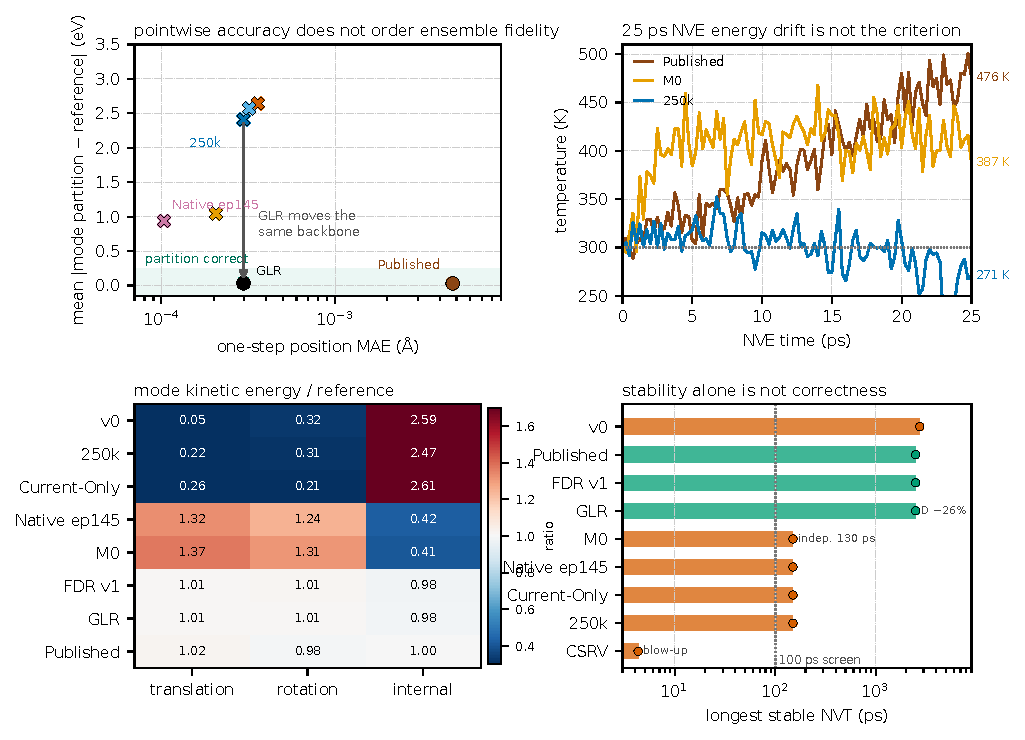
\includegraphics[width=\linewidth]{fig1_diagnostic.pdf}
  \caption{Pointwise accuracy and short-horizon stability do not predict NVT fidelity.
  (a) One-step position error versus mean absolute mode-partition error. The published checkpoint
  has a large one-step error but a correct partition; the 250k model is pointwise better and fails.
  The GLR moves the same 250k backbone to a correct partition without changing its position head.
  (b) 25 ps NVE temperature traces. (c) Mode kinetic energy relative to the reference NVT.
  (d) Longest stable NVT run and the partition verdict.}
  \label{fig:diagnostic}
\end{figure}

\subsection{A mode-resolved generalized Langevin readout}

\textbf{Framework.} The method has one fixed readout and two plug-ins: the frozen backbone
\(f_\theta\) and the physics-defined mode basis \(\mathcal M\). The readout algorithm is fixed:
(i) decompose the velocity into the modes in \(\mathcal M\); (ii) fit an AR(10) process to each
mode's reference ACF by Yule--Walker; (iii) add FD-consistent noise; (iv) blend with the backbone
velocity at \(\lambda=0.1\); (v) rescale each group to its canonical kinetic energy
(\(N_a k_BT/2\) in the deterministic limit, Gamma-distributed in the stochastic configuration);
(vi) project out the total centre-of-mass velocity. The position update is always
\(q_{t+1}=q_t+\Delta q_t\). The rest of the paper instantiates \(\mathcal M\) as molecular
translation/rotation/internal modes for water and as phonon bands for quartz, with a species
partition as a coarser control; the readout itself does not change. For quartz the memory kernel
is switched off because the 5 fs backbone already reproduces the phonon ACF; only the
variance-rescale component is active.

The diagnostic says that the missing object is a mode-resolved stationary measure. We therefore
leave the backbone unchanged and add a readout whose job is to enforce that measure. The
architecture is deliberately asymmetric. The frozen backbone supplies the displacement
\(\Delta q_t\); the readout supplies the velocity \(v_t\) that enters the next backbone call and
the kinetic diagnostics. The position update remains
\begin{equation}
q_{t+1}=q_t+\Delta q_t,
\end{equation}
so the learned displacement stays in distribution and the readout is not integrated as a second
position update. We tested the obvious alternative---adding the velocity correction to the
displacement---and it crashed at 24.8 ps (minimum interatomic distance 0.647 \AA), confirming that
the decoupling is a stability requirement rather than a stylistic choice.

The readout decomposes the velocity into molecular translation, rotation, and internal modes,
which are orthogonal under the mass-weighted inner product (Methods). For each mode, an AR(\(p\))
process is fitted to the reference velocity ACF by Yule--Walker; the prediction-error ratio
\(\rho_a\) sets the FD noise variance, \(\operatorname{Var}(\varepsilon^a)=\rho_a N_a k_BT/2\).
The AR prediction and the noise are blended with the backbone velocity,
\(v_t^{\rm blend}=(1-\lambda)v_t^{\rm pred}+\lambda\tilde v_t\) with \(\lambda=0.1\), and each mode
is rescaled to its canonical mean kinetic energy,
\begin{equation}
v_t^{\rm GLR}=\sum_a s_a\,(v_t^{\rm blend})^a,\qquad
s_a=\sqrt{\frac{N_a k_BT/2}{\tfrac12\sum_i m_i|(v_t^{\rm blend})_i^a|^2}}.
\end{equation}
The total centre-of-mass velocity is projected out after the rescale. The construction guarantees
the canonical mode/group kinetic-energy marginal (mean \(N_a k_BT/2\), Gamma-distributed in the stochastic configuration) at every step and the AR(\(p\)) stationary ACF up to lag
\(p\). The position marginal is not guaranteed analytically; it is learned by the backbone and
validated empirically. The per-step rescale suppresses the mode-KE fluctuations (reference std
about 0.24 eV versus about 0.002 eV), so the guarantee is on the first moment; the marginal
velocity distribution is nevertheless close to the reference (component kurtosis
2.93/5.49/5.93 versus 3.04/5.62/5.57 for translation, rotation, and internal motion). Throughout,
``thermodynamically consistent'' refers to this mean-partition-plus-ACF guarantee, not the full
joint distribution or exact transport; the 26\% diffusion deficit is reported as a transport
limitation.

The order \(p\) is the only structural knob. AR(1) matches the 5 fs correlation but not the
25--100 fs memory and produces the wrong O--H RDF; AR(10) matches the short- and mid-lag ACF;
AR(20) also captures the 100--200 fs internal tail. The main configuration uses AR(10); the order
sweep is an ablation. The readout is fitted, not trained: it needs a short reference NVT
trajectory (100 ps here), but no backbone gradients, forces, or new labels. The next section
applies it to the same frozen 250k backbone that failed the NVT screen without it.

\begin{figure}[t]
  \centering
  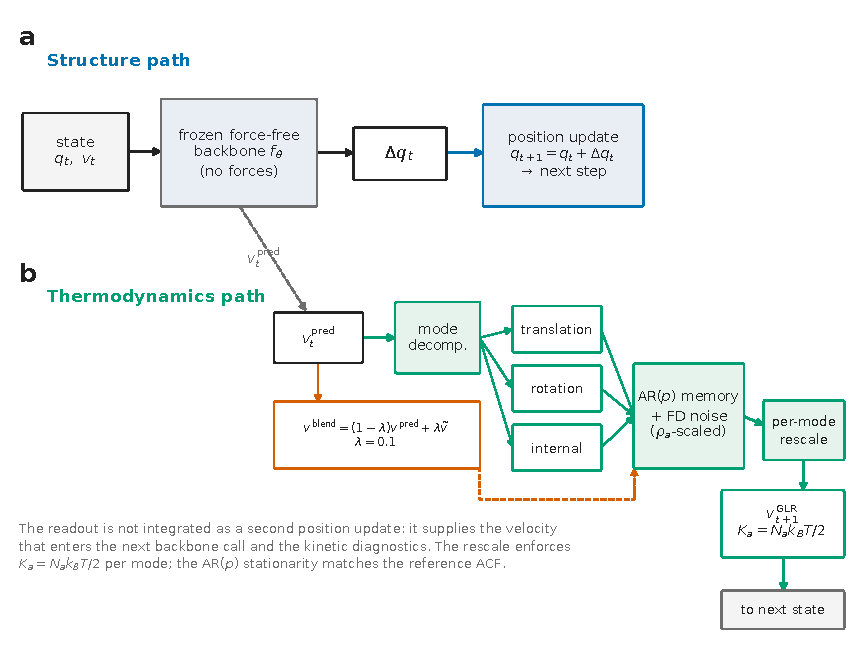
\includegraphics[width=\linewidth]{fig2_architecture.pdf}
  \caption{The GLR architecture. The frozen backbone supplies the displacement; the readout
  supplies the velocity that enters the next backbone call. The AR(\(p\)) memory kernel is fitted
  from the reference ACF, the FD noise variance follows from the prediction error, and the
  per-mode rescale enforces \(K_a=N_a k_BT/2\). The readout is not integrated as a second position
  update.}
  \label{fig:architecture}
\end{figure}

\subsection{Water NVT}

We applied the GLR to the frozen 250k backbone that failed the NVT screen without it. The readout
was fitted once from a 100 ps block of the reference NVT trajectory (500--600 ps) and then used
unchanged in all rollouts. We ran 100 ps from the val\_04 NVE initial condition and from an
independent NVT trajectory (301.8 K), and a 2.5 ns production run from each start. The integration
step is 5 fs; no external thermostat is applied---the GLR is the thermostat. We compare the mode
kinetic partition, the mode velocity ACFs, the O--O/O--H/H--H RDFs, the H/O VDOS, and the molecular
centre-of-mass MSD and diffusion coefficient against the reference NVT trajectory.

Without the readout, the 250k backbone has translation \(0.538\) eV, rotation \(0.786\) eV, and
internal \(6.044\) eV. With the GLR, the 100 ps partition is \(2.482/2.526/2.399\) eV from val\_04
and \(2.445/2.490/2.362\) eV from the independent start, against the 2.5 ns reference means of
\(2.459/2.502/2.450\) eV. The total temperature is 300.0 K in both runs. The 2.5 ns runs give
\(2.482/2.526/2.399\) and \(2.482/2.527/2.398\) eV. The two starts agree within the reference
block-to-block scatter, so the stationary partition is not a property of the val\_04 initial
condition. The published checkpoint gives \(2.505/2.463/2.444\) eV, also correct but with a
different mix of residuals.

The per-mode ACFs tell the same story. The translation ACF matches the reference at 5, 25, 100,
and 500 fs (GLR 0.981/0.640/0.014/\(-0.030\) versus reference 0.982/0.658/0.039/\(-0.019\)). The
internal ACF matches at 5 fs (\(-0.575\) versus \(-0.567\)) and reproduces the mid-lag oscillation;
the 500 fs tail is still too persistent (0.312 versus 0.104), a known limitation of AR(10). The
AR(20) fit removes most of that residual (internal 100/200 fs 0.147/0.068 versus 0.147/0.072) and
is reported as an order ablation rather than the main configuration. The readout matches the
multi-lag dynamics, not just a single 5 fs gain. The ACF match is by construction from the fit and
is therefore not an independent validation; the RDF, VDOS, and diffusion are the independent
tests.

The 100 ps RDFs are closer to the reference than the published checkpoint in our analysis:
O--O 0.032 versus 0.043, O--H 0.104 versus 0.118, H--H 0.026 versus 0.096. The independent start
gives 0.036/0.098/0.027, essentially the same. The O VDOS overlap is 0.964 versus 0.937 for the
published checkpoint; the H VDOS overlap is 0.848 versus 0.624. The H comparison is sensitive to
our reference H-stretch frequency (the published model scores 0.624 here while the paper reports
about 0.99 with its own reference), so we treat the O VDOS and the RDFs as the robust comparisons
and report the H number with that caveat. At 2.5 ns the RDFs improve further to
O--O 0.031, O--H 0.038, and H--H 0.028, and the O VDOS is 0.953; the longer run resolves the
O--H distribution more accurately than the 100 ps screen.

The improvement over the AR(1) readout is large and diagnostic. FDR v1, which has the correct
partition but only a single gain, gives O--O 0.062, O--H 0.301, H--H 0.110 and H/O VDOS 0.807/0.851.
The AR(10) memory kernel improves O--H by a factor of 2.6 and the H VDOS by five points. The
memory order, not the global temperature, is what controls the O--H spectrum.

The 2.5 ns run remains stable (temperature 299.99 K, minimum interatomic distance above 0.93 \AA)
and shows no sign of the slow collective drift that characterized the un-readout models. The
8-block diffusion analysis gives \(D=1.406\pm0.155\times10^{-9}\) m\(^2\) s\(^{-1}\), against
\(1.883\pm0.306\times10^{-9}\) for the reference: the GLR is 26\% low. The published checkpoint is
16\% high (2.18\(\times10^{-9}\)). The FDR v1 fast tail (3.59\(\times10^{-9}\)) is absent, so the
GLR fixes the qualitative failure of the AR(1) readout but undershoots the reference. The
independent 2.5 ns run gives an essentially identical result: partition
\(2.482/2.527/2.398\) eV, RDFs 0.028/0.044/0.027, H/O VDOS 0.847/0.953, and
\(D=1.393\pm0.079\times10^{-9}\). The two 2.5 ns starts agree on the stationary measure, including
the 26\% diffusion deficit; the deficit is a property of the decoupled architecture, not of the
initial condition.

A stochastic-target variant of the same readout gives the same partition and MSD diffusion
(1.435/1.387\(\times10^{-9}\)) and restores the total kinetic-energy variance (0.437/0.429 versus
0.440 eV), but its Green--Kubo integral is \(1.16\times10^{-9}\), inconsistent with the MSD
\(1.44\times10^{-9}\). The deterministic target is therefore used for production: it preserves
the GK--MSD consistency that identifies the transport deficit as a translation-ACF effect.

The Green--Kubo integral of the mass-weighted translation ACF gives 1.42\(\times10^{-9}\) for the
GLR and 1.84\(\times10^{-9}\) for the reference, in agreement with the MSD values. The position
update is therefore consistent with the readout velocity; the deficit is in the translation ACF
integral. The AR(10) translation ACF is \(-0.032\) at 100 fs while the reference is \(+0.039\);
the AR(20) fit matches this lag. A mixed readout with translation AR(20) and rotation/internal
AR(10) raises the Green--Kubo estimate to 1.61\(\times10^{-9}\) at 100 ps but does not close the
MSD gap. We also tested translation-blend, translation-displacement, and molecule-COM scaling
variants; none closed the gap without breaking the MSD--Green--Kubo consistency or the RDF
(Supplementary Information). The decoupled position update remains the limiting factor; we report
the 26\% deviation as a limitation rather than claiming exact diffusion recovery.

The GLR is the first configuration in this study that combines (i) a stable 2.5 ns NVT run,
(ii) a canonical mean mode/group kinetic-energy partition, (iii) multi-lag ACF agreement, and
(iv) RDF and VDOS at or beyond the published checkpoint. Its diffusion coefficient is 26\% low but
qualitatively correct, and far closer than the AR(1) readout. It does so with a frozen backbone and
a readout fitted from 100 ps of reference data. The remaining questions---the internal long tail
and the diffusion deficit---are addressed in the ablations and discussion; the second system is
quartz (Section 2.5).

\begin{figure}[t]
  \centering
  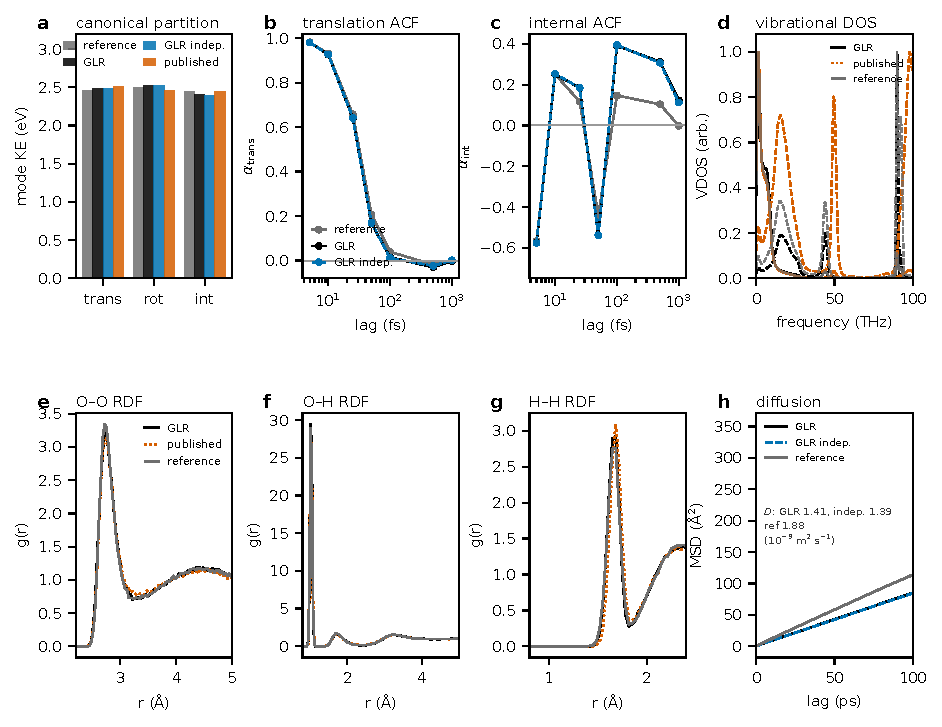
\includegraphics[width=\linewidth]{fig3_water.pdf}
  \caption{Water NVT results. (a) Mode kinetic partition. (b, c) Translation and internal ACFs.
  (d) Vibrational DOS (normalized). (e--g) O--O, O--H, and H--H RDFs. (h) Molecular-COM MSD and the
  2.5 ns diffusion. Panels (a--g) are 100 ps, so the RDF/VDOS comparison with the published
  checkpoint is length-matched; panel (h) is 2.5 ns for both GLR starts and the reference.}
  \label{fig:water}
\end{figure}

% Table 1 — long-time NVT comparison. Values from our 100 ps / 2.5 ns screens.
% Diffusion for GLR is a placeholder until the 2.5 ns analysis finishes.
\begin{table*}[t]
\centering
\small
\caption{Long-time NVT behaviour of force-free propagators and readouts on SPC/Fw water.
Partition is translation/rotation/internal kinetic energy; the reference is the 2.5 ns NVT mean
(2.459/2.502/2.450 eV). The first 100 ps reference block is an outlier (2.373/2.430/2.609 eV);
using it would exaggerate the GLR/published residuals but not change the ranking. RDF is RMSE
against the reference NVT; VDOS is the overlap. RDF/VDOS columns are 100 ps for all rows except
the GLR 2.5 ns row; this keeps the published comparison length-matched. Diffusion is from 2.5 ns
rollouts where available (the 100 ps GLR row shows the seed range). ``Stable'' is the longest NVT
run without a safety stop; a stable run can still have the wrong partition.}
\label{tab:comparison}
\resizebox{\linewidth}{!}{%
\begin{tabular}{@{}lcccccc@{}}
\toprule
Method & Stable NVT & Partition (eV) & O--O / O--H / H--H RDF & VDOS (H/O) & $D$ ($10^{-9}$ m$^2$ s$^{-1}$) & Verdict \\
\midrule
Reference & 2.5 ns & 2.459 / 2.502 / 2.450 & 0 / 0 / 0 & 1 / 1 & 1.84--1.88 & --- \\
v0 & 2.75 ns & 0.111 / 0.808 / 6.338 & 0.944 / 1.409 / 0.229 & 0.356 / 0.236 & 0.0003 & fail \\
250k & 150 ps & 0.538 / 0.786 / 6.044 & 0.646 / 1.312 / 0.249 & 0.406 / 0.487 & --- & fail \\
Current-Only & 150 ps & 0.646 / 0.535 / 6.384 & 0.631 / 1.345 / 0.232 & 0.348 / 0.600 & --- & fail \\
Native ep145 & 150 ps & 3.256 / 3.105 / 1.041 & 0.180 / 1.584 / 0.074 & 0.683 / 0.905 & --- & fail \\
M0 & 150 ps & 3.373 / 3.270 / 1.000 & 0.191 / 1.790 / 0.082 & 0.668 / 0.888 & --- & fail$^a$ \\
FDR v1 (AR1) & 2.5 ns & 2.482 / 2.533 / 2.392 & 0.062 / 0.301 / 0.110 & 0.807 / 0.851 & 3.59 & pass \\
GLR (AR10) & 100 ps & 2.482 / 2.526 / 2.399 & 0.032 / 0.104 / 0.026 & 0.848 / 0.964 & 1.20--1.45 & pass \\
\textbf{GLR (AR10)} & \textbf{2.5 ns} & \textbf{2.482 / 2.526 / 2.399} & \textbf{0.031 / 0.038 / 0.028} & \textbf{0.847 / 0.953} & \textbf{1.39--1.41} & \textbf{pass}$^b$ \\
Published TrajCast & 2.5 ns & 2.505 / 2.463 / 2.444 & 0.043 / 0.118 / 0.096 & 0.624 / 0.937 & 2.18 & pass \\
\bottomrule
\end{tabular}}
\begin{flushleft}
\footnotesize
$^a$M0 passes on the val\_04 start but blows up at 130 ps on an independent start.\\
$^b$GLR diffusion is 26\% below the reference on two starts (independent 2.5 ns: RDF
0.028/0.044/0.027, VDOS 0.847/0.953, D 1.39); partition, RDF, and VDOS pass. A stochastic-target
2.5 ns variant restores the KE variance (0.437/0.429 versus 0.440 eV) but its Green--Kubo integral
is \(1.16\times10^{-9}\), inconsistent with the MSD \(1.44\times10^{-9}\); it is reported as an
ablation, and the deterministic target is used for production.\\
H VDOS overlap is sensitive to the reference H-stretch frequency; O VDOS and the RDFs are the
robust comparisons.\\
\end{flushleft}
\end{table*}


\subsection{The readout is backbone-agnostic}

The GLR is fitted from the reference ACF and does not depend on the backbone architecture in
principle. To test this empirically, we applied the same AR(10) coefficients and the same
\(\lambda=0.1\) blend to the v0 phase-space operator, a different propagator (3.04M parameters)
that fails the NVT screen even more strongly than the 250k model. Without the readout, v0 gives
translation/rotation/internal \(0.111/0.808/6.338\) eV, RDF RMSEs 0.944/1.409/0.229, and H/O VDOS
0.356/0.236. With the GLR it is stable at 300.0 K, with partition
\(2.482/2.529/2.396\) eV, RDF 0.042/0.109/0.019, and H/O VDOS 0.855/0.969 (Table~\ref{tab:backbones}).
The structure and spectra are comparable to the 250k GLR (0.032/0.104/0.026; 0.848/0.964), despite
the different backbone. The independent start gives the same partition (2.482/2.527/2.398), RDF
0.050/0.131/0.023, and H/O VDOS 0.857/0.977, so the rescue is not a val\_04 artifact. The readout
is therefore empirically backbone-agnostic across two architectures, not just a correction tuned
to one model.

% Table 3 — Backbone-agnostic test: v0 phase-space vs 250k relational.
\begin{table}[t]
\centering
\small
\caption{The same GLR coefficients applied to two different frozen backbones. The v0 phase-space
operator fails the NVT screen without the readout; with the GLR it becomes stable and partitioned,
with structure and VDOS comparable to the 250k relational backbone. All rows are 100 ps;
the reference partition is the 2.5 ns mean.}
\label{tab:backbones}
\resizebox{\linewidth}{!}{%
\begin{tabular}{@{}lcccc@{}}
\toprule
Backbone & Readout & Partition (eV) & O--O / O--H / H--H RDF & H / O VDOS \\
\midrule
250k relational (2.36M) & none & 0.538 / 0.786 / 6.044 & 0.646 / 1.312 / 0.249 & 0.406 / 0.487 \\
250k relational (2.36M) & GLR & 2.482 / 2.526 / 2.399 & 0.032 / 0.104 / 0.026 & 0.848 / 0.964 \\
v0 phase-space (3.04M) & none & 0.111 / 0.808 / 6.338 & 0.944 / 1.409 / 0.229 & 0.356 / 0.236 \\
v0 phase-space (3.04M) & GLR & 2.482 / 2.529 / 2.396 & 0.042 / 0.109 / 0.019 & 0.855 / 0.969 \\
\bottomrule
\end{tabular}}
\vspace{2pt}
\begin{flushleft}
\footnotesize
v0 + GLR independent start: partition 2.482/2.527/2.398 eV; RDF 0.050/0.131/0.023;
H/O VDOS 0.857/0.977. The rescue is not specific to val\_04.
\end{flushleft}
\end{table}


\subsection{Cross-material limit: quartz}

To test the readout beyond molecular liquids, we applied a phonon-band variance rescale to
crystalline quartz (162 atoms) with a 5 fs backbone trained on the same NVE data and the 15 ns
NVT reference. The 5 fs baseline cools to 235.3 K (species KE 0.0298/0.0305 eV per atom), with
Si--O RDF RMSE 0.271 and O/Si VDOS overlaps 0.918/0.944 (Table~\ref{tab:quartz}). The stochastic
phonon-band rescale (two seeds) sets \(T=299.8/299.9\) K, reproduces the total kinetic-energy
standard deviation (0.397/0.399 versus 0.4017 eV), gives Si/O KE 0.03846/0.03855 eV per atom,
improves the Si--O RDF to 0.0245/0.0312, and preserves the O/Si VDOS at 0.953/0.949 and
0.947/0.962. The seed means are \(T=299.9\) K, KE std 0.398 eV, Si--O RDF 0.028, and VDOS
0.950/0.955. A coarser species partition
gives \(T=301.68\) K, exact Si/O equipartition (0.03872/0.03877 eV), total KE std 0.4012 eV,
VDOS 0.898/0.955, and the same Si--O RDF, showing that the result is robust to the coarse
partition. The deterministic species rescale is an ablation: it fixes the mean but suppresses the
kinetic-energy variance (0.0036 eV) and gives VDOS 0.866/0.914. The full species GLR (memory +
noise) is a negative control: the species basis is not a phonon eigenbasis, and the readout
collapses the VDOS to 0.07 even at 5 fs. To test whether a physically correct basis rescues the
memory kernel, we built a 486-mode phonon basis from a finite-difference Hessian of the same
potential and ran a per-mode AR(10) GLR. The phonon basis is canonical (99.4\% of modes within
10\% of \(k_BT/2\) over 2 ns), but the 5 fs backbone's mode ACF is already correct; the AR
innovations broaden the sharp phonon lines and reduce the VDOS to 0.734/0.838. A 30 fs backbone
shows the same pattern more strongly (ACF prediction error 0.91; full GLR VDOS 0.225;
deterministic rescale 0.838/0.835). The variance-rescale component therefore generalizes across a
covalent solid; the memory kernel is useful only when the backbone's mode ACF is wrong. Quartz's
failure is a variance bias, not a memory deficit.

% Table 4 — Cross-material: quartz at 5 fs, phonon-band stochastic variance rescale.
\begin{table}[t]
\centering
\small
\caption{Cross-material test. The 5 fs quartz backbone is trained on the same NVE data and
evaluated against the 15 ns NVT reference. The phonon-band stochastic variance rescale sets the
canonical temperature and total kinetic-energy variance, improves the Si--O RDF, and preserves
the phonon VDOS. The quoted band row is the mean of two seeds (T=299.8/299.9 K; VDOS O/Si
0.953/0.949 and 0.947/0.962; mode KE within 10\% 78.1\%/76.2\%). A coarser species partition gives statistically consistent structure and VDOS
with exact Si/O equipartition. The deterministic rescale is an ablation: it fixes the mean but
suppresses the kinetic-energy variance. The full species GLR (memory + noise) and the full
phonon-mode GLR are negative controls. The phonon-mode control uses the correct eigenbasis, but
the 5 fs backbone's mode ACF is already correct, so the AR innovations broaden the phonon lines.
The 30 fs deterministic row is shown for the horizon comparison; its kinetic-energy variance was
not measured.}
\label{tab:quartz}
\resizebox{\linewidth}{!}{%
\begin{tabular}{@{}lccccc@{}}
\toprule
Quartz & $T$ (K) & KE std (eV) & Si/O KE per atom (eV) & RDF Si--O / O--O / Si--Si & VDOS O / Si \\
\midrule
5 fs baseline & 235.3 & 0.4355 & 0.0298 / 0.0305 & 0.271 / 0.096 / 0.133 & 0.918 / 0.944 \\
\textbf{5 fs phonon-band stochastic rescale} & \textbf{299.9} & \textbf{0.398} & \textbf{0.03846 / 0.03855} & \textbf{0.028 / 0.016 / 0.033} & \textbf{0.950 / 0.955} \\
5 fs species stochastic rescale (control) & 301.68 & 0.4012 & 0.03872 / 0.03877 & 0.0245 / 0.0169 / 0.0380 & 0.898 / 0.955 \\
5 fs deterministic species rescale (ablation) & 301.86 & 0.0036 & 0.03878 / 0.03878 & 0.078 / 0.022 / 0.055 & 0.866 / 0.914 \\
5 fs full species GLR (negative) & 301.86 & --- & 0.03878 / 0.03878 & 0.529 / 0.263 / 0.441 & 0.074 / 0.067 \\
5 fs full phonon GLR (negative) & 301.9 & 0.4024 & 0.03872 / 0.03877 & 0.197 / 0.044 / 0.083 & 0.734 / 0.838 \\
30 fs deterministic rescale & 301.9 & --- & 0.03878 / 0.03878 & 0.149 / 0.024 / 0.051 & 0.838 / 0.835 \\
\bottomrule
\end{tabular}}
\end{table}


\subsection{Cost and reference-data efficiency}

The GLR adds a mode decomposition and a \(p\)-step history per step; the cost is negligible
compared with the backbone. On water the end-to-end rollout is 15.4 ns day\(^{-1}\) on an RTX
PRO 6000 with 185 MB peak memory, and the 250k backbone dominates the runtime. The readout is
fitted from 100 ps of reference NVT; refitting on a different 100 ps block changes the AR
coefficients by at most 0.08 (correlation 0.999), so the reference-data requirement is small and
stable. Backbone training, not the readout, is the dominant cost. A full scalability sweep across
system size and horizon is left to the Supplementary Information.

\subsection{Ablations}

The AR-order ablation uses the deterministic target to isolate the kernel order; the main
configuration uses the stochastic target. The AR(1) readout is the natural minimal thermostat:
one gain per mode, fitted to the 5 fs correlation. It holds the mean partition once the variance is rescaled, but it does not reproduce
the multi-lag dynamics. At 100 ps, the O--H RDF RMSE is 0.312 for the GLR AR(1), 0.301 for FDR v1,
0.131 for AR(5), 0.104 for AR(10), and 0.117 for AR(20); the O--H RDF is the clearest signature.
The AR(1) internal ACF decays monotonically from \(-0.567\) to zero, while the reference oscillates
and crosses zero near 25 fs; the AR(10) kernel reproduces the oscillation. The AR(20) kernel also
captures the 100--200 fs tail (internal 100/200 fs 0.147/0.068 versus 0.147/0.072), at the cost of
a longer history and a larger coefficient vector, but its better long-lag ACF does not translate
into a better short-window O--H. AR(10) therefore remains the main configuration; the order sweep
shows the qualitative improvement from AR(1) to AR(10) rather than a monotone gain with order.

The ablation that removes the per-step rescale isolates the partition guarantee. In the AR(1)
readout, removing the rescale collapses the total kinetic energy and cools the system to about
14 K. With the GLR readout, the no-rescale run is stable but cools to 172 K; the partition is
0.763/0.649/2.839 eV, the RDFs degrade to 0.398/0.474/0.279, and the H/O VDOS overlaps fall to
0.432/0.608. The rescale is not a cosmetic normalization; it is the step that makes the mode
kinetic energy a design constraint rather than a by-product of the backbone and the noise.

Contrary to our expectation, removing the FD noise did not degrade the 100 ps structure:
the partition is unchanged (\(2.482/2.526/2.399\) eV), the RDFs are 0.034/0.098/0.026, the
H/O VDOS overlaps are 0.849/0.962, and the 10--80 ps diffusion estimate is 1.55\(\times10^{-9}\)
(versus 1.45\(\times10^{-9}\) with noise). At the small blend \(\lambda=0.1\), the backbone and
the variance rescale provide enough fluctuation that the noise term is not the empirical driver.
The memory kernel and the rescale are the load-bearing components; the FD noise is part of the
theoretical construction and may matter at larger blend or for the one-point velocity
distribution, but we do not claim it is necessary on the basis of this ablation.

For the AR(1) readout, increasing the internal blend from 0.1 to 1.0 makes the O--H RDF worse
(0.957 versus 0.301) and the VDOS worse (H/O 0.618/0.613 versus 0.807/0.851). A larger admixture
of a single-gain readout does not fix the spectrum; it replaces the backbone's internal bias with
the readout's wrong long-lag dynamics. The blend is kept at 0.1 to preserve the position head; the
memory kernel, not the blend, does the work.

Adding the velocity correction to the displacement---the obvious way to make positions and
velocities consistent---crashes at 24.8 ps (minimum distance 0.647 \AA) while the temperature
remains at 300 K. The failure is structural, not thermal: the correction injects a displacement
increment that the backbone's next state cannot absorb. The decoupled scheme is therefore a
stability requirement, and the method does not simply integrate the readout velocity.

Three 100 ps seeds give the same partition (2.482/2.526/2.399 eV) and a narrow spread in the
structural metrics: O--H 0.104/0.111/0.110, O--O 0.032/0.034/0.033, H VDOS 0.848/0.854/0.846,
and O VDOS 0.964/0.966/0.959. The 2.5 ns O--H improvement to 0.038 is therefore a sampling effect
of the longer trajectory, not a seed fluctuation. The 100 ps diffusion estimates are noisier:
1.20/1.21/1.45\(\times10^{-9}\) across the three seeds (10--80 ps fit). The two 2.5 ns runs give
1.39--1.41\(\times10^{-9}\), within the seed spread and far more stable; the 26\% deficit is
therefore robust, but the 100 ps \(D\) should not be over-interpreted. The frozen-vs-end-to-end backbone comparison remains future work;
the present paper tests two frozen backbones and two materials, and the claim is architectural
rather than universal.

\begin{figure}[t]
  \centering
  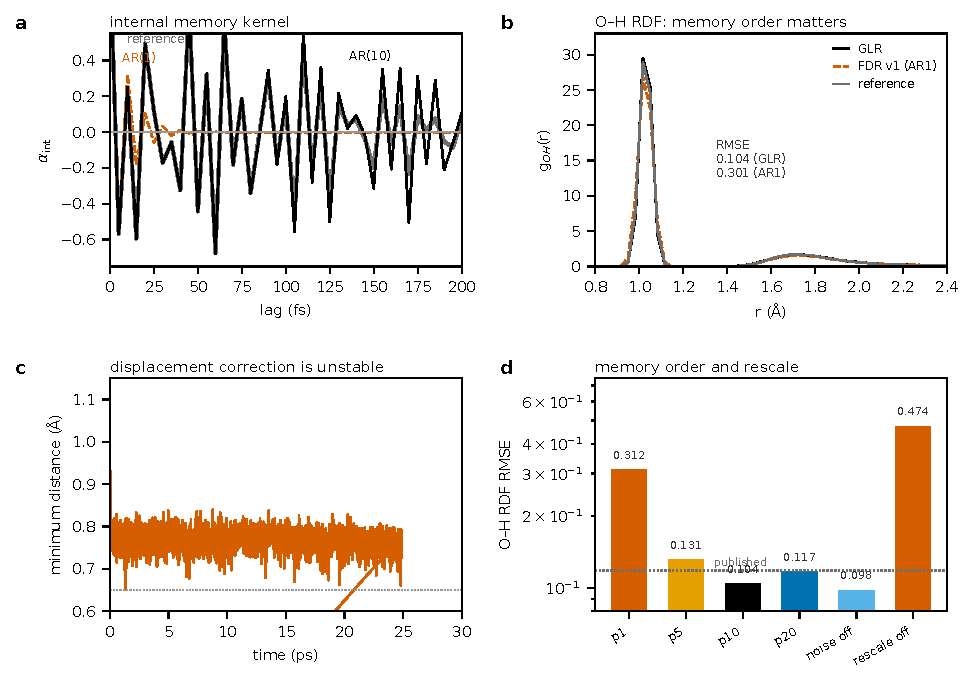
\includegraphics[width=\linewidth]{fig4_ablations.pdf}
  \caption{Ablations. (a) Internal ACF for AR(1) and AR(10) against the reference. (b) O--H RDF
  for the AR(1) and AR(10) readouts. (c) Minimum interatomic distance for the direct
  displacement-correction variant, which stops at 24.8 ps. (d) O--H RDF for the AR order,
  noise-off, and rescale-off ablations; the dashed line is the published checkpoint.}
  \label{fig:ablations}
\end{figure}
